\documentclass[14pt]{extarticle}
\usepackage[utf8]{inputenc}
\usepackage{amsmath}
\usepackage{amsfonts}
\usepackage{graphicx}
\usepackage{setspace}
\usepackage{geometry}
\usepackage{enumitem}
\usepackage{amssymb}
\usepackage{xcolor}
\usepackage{mathtools}
\usepackage{float}
\usepackage{listings}
\usepackage{tabularx}

\geometry{
    top=1in,
    bottom=1in,
    left=1in,
    right=1in,
    headheight=14pt,
    headsep=25pt,
    footskip=30pt
}

\title{Bayes Theorem}
\author{Yana Jin}
\date{Wednesday, 24th September 2024}

\onehalfspacing

\newcommand{\coverpage}{%
    \begin{titlepage}
        \centering
        
\includegraphics[width=1\textwidth]{cover.png}
    \end{titlepage}
}

\begin{document}

\coverpage

\newpage

\section*{Multiple Linear Regression}

\noindent
Recall simple linear regression 
\[
E(Y|X_1 = x_1) = \beta_0 + \beta_1 x_1
\]
Now suppose we have a second variable $X_2$
Consider the model:
\[
E(Y|X_1 = x_1, X_2 = x_2) = \beta_0 + \beta_1 x_1 + \beta_2 x_2
\]
Idea: use $X_2$ to help explain part of (the variation in) $Y$ not already explained by $X_1$.

\section*{United Nations Fertility Data}

\noindent
\textit{lifeExpF} = life expectancy (response)\\
\textit{fertility} = birth rate per 1000 females from 2009

\noindent
\textit{ppgdp} = GDP per person in USD

\bigskip

\noindent
Data from 199 UN member countries and a few others (e.g., Hong Kong) \\
\textit{[Data collected in 2011]}
\begin{figure}[H]
    \centering
    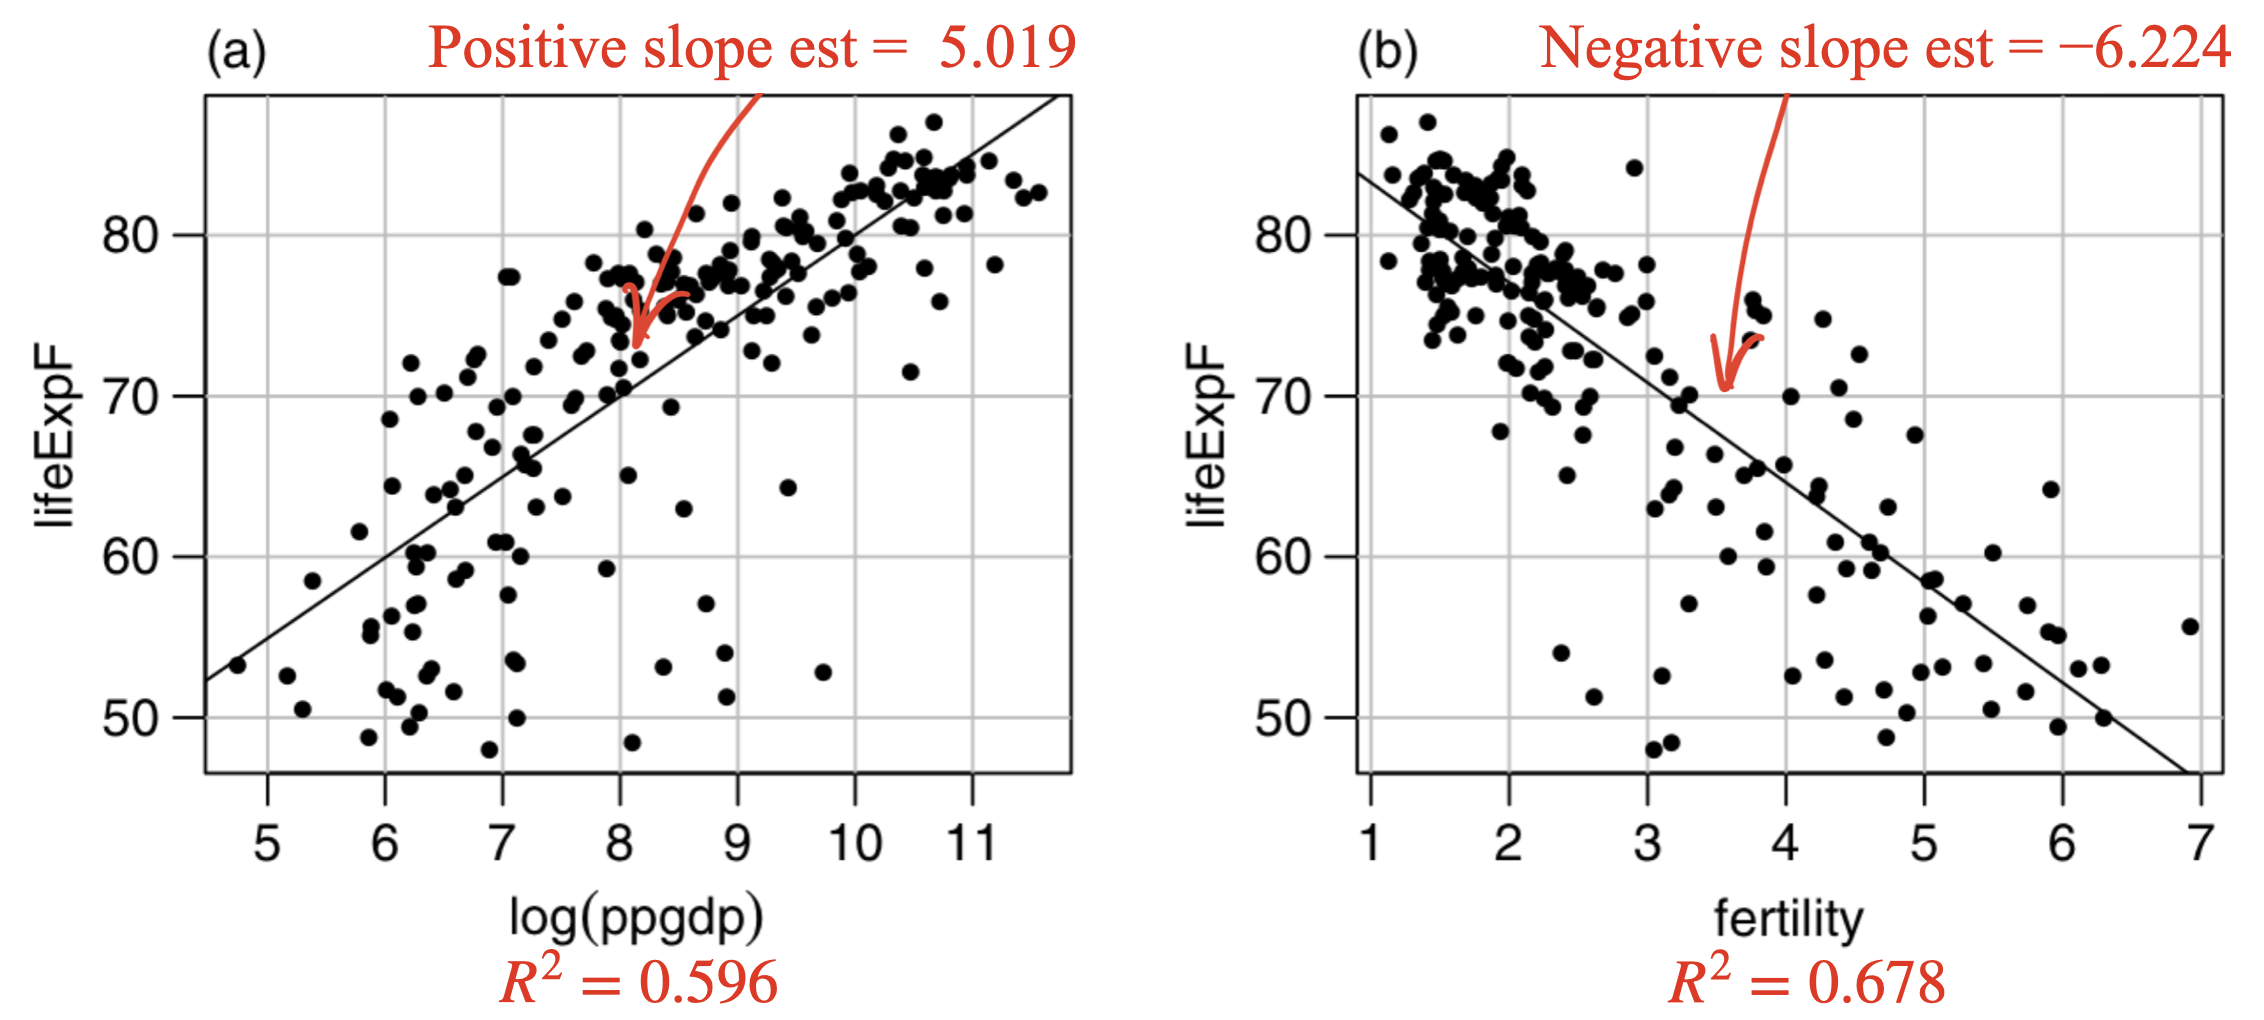
\includegraphics[width=1\textwidth]{fig1.png}
\end{figure}

\noindent
\textcolor{blue}{\textbf{Fact:} If $\log(\text{ppgdp})$ and fertility were uncorrelated, above figure would provide a complete summary of the dependence of response on regressors.}
\begin{figure}[H]
    \centering
    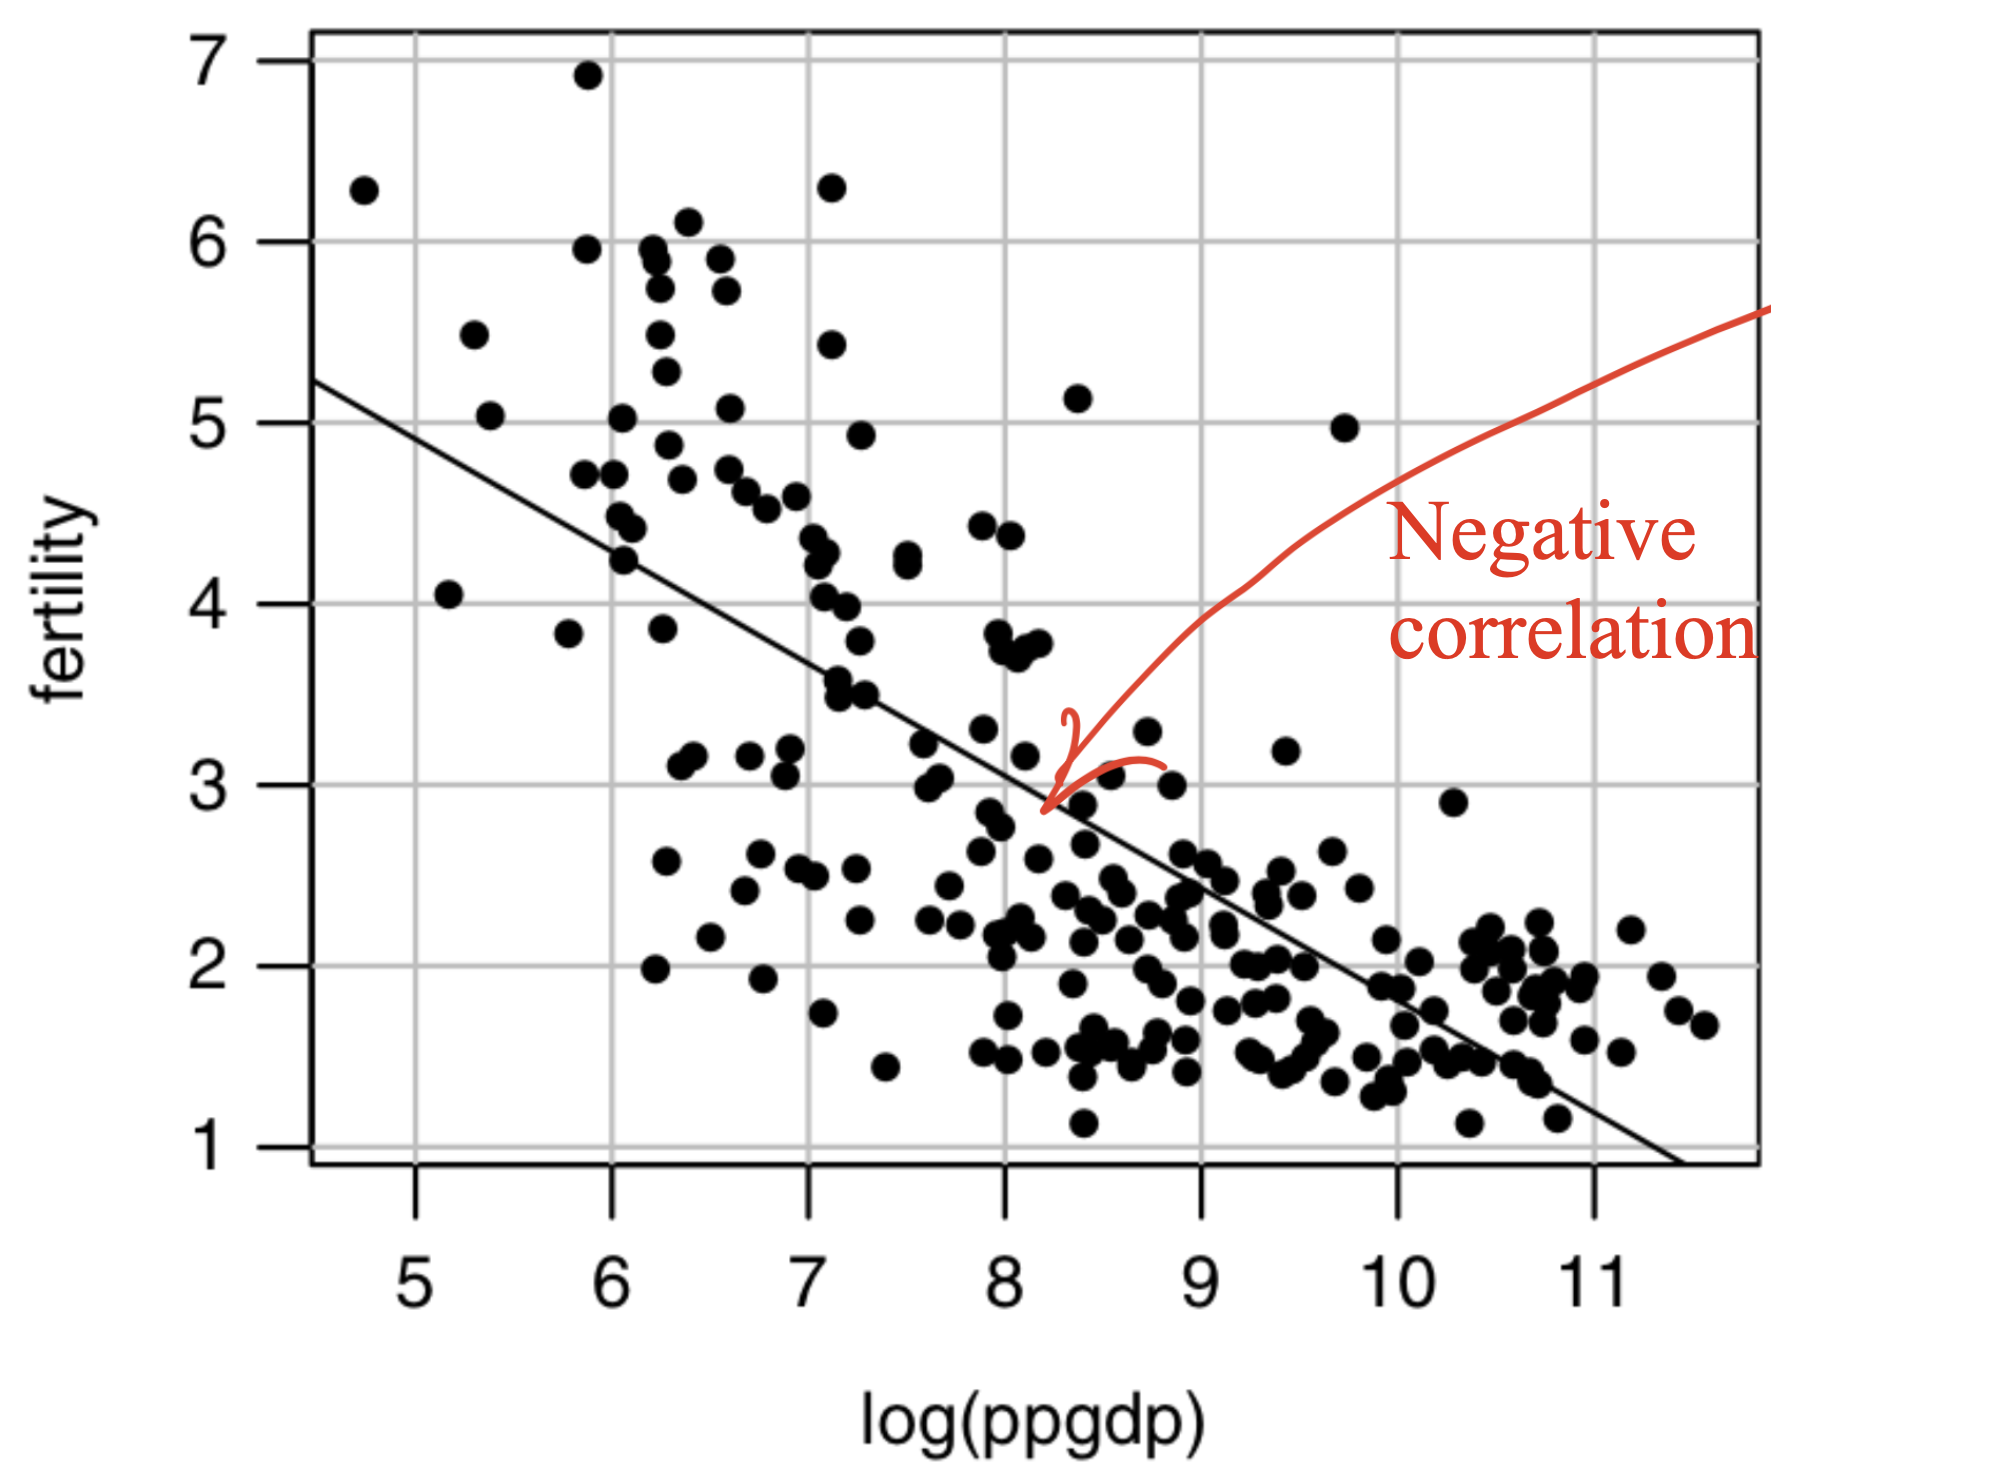
\includegraphics[width=0.8\textwidth]{fig2.png}
\end{figure}

\noindent
\textcolor{red}{$\Longrightarrow$ The regressors will in part be explaining the same variation in lifeExpF.}

\section*{Intuition About Explained Variability}

\noindent
Total explained variation explained jointly by two variables $X_1, X_2$ can take different scenarios:\\
1) If population correlation $\rho(X_1, X_2) = 0$, then variation explained jointly = sum of variations explained individually.\\
2) If $\rho(X_1, X_2) \neq 0$, then the situation is more complicated \\
\quad -- total variation can exceed or be less than the sum of individual variation.

\section*{Added Variable Plots}
Used to get the effect of adding in $X_2$ to a model that already includes $X_1$.\\
Let's consider the fertility dataset again.\\
\textbf{Steps}\\
1. Compute regression of lifeExpF on $\log(\text{ppgdp})$ \textcolor{red}{(see Fig. below)}
\begin{figure}[H]
    \centering
    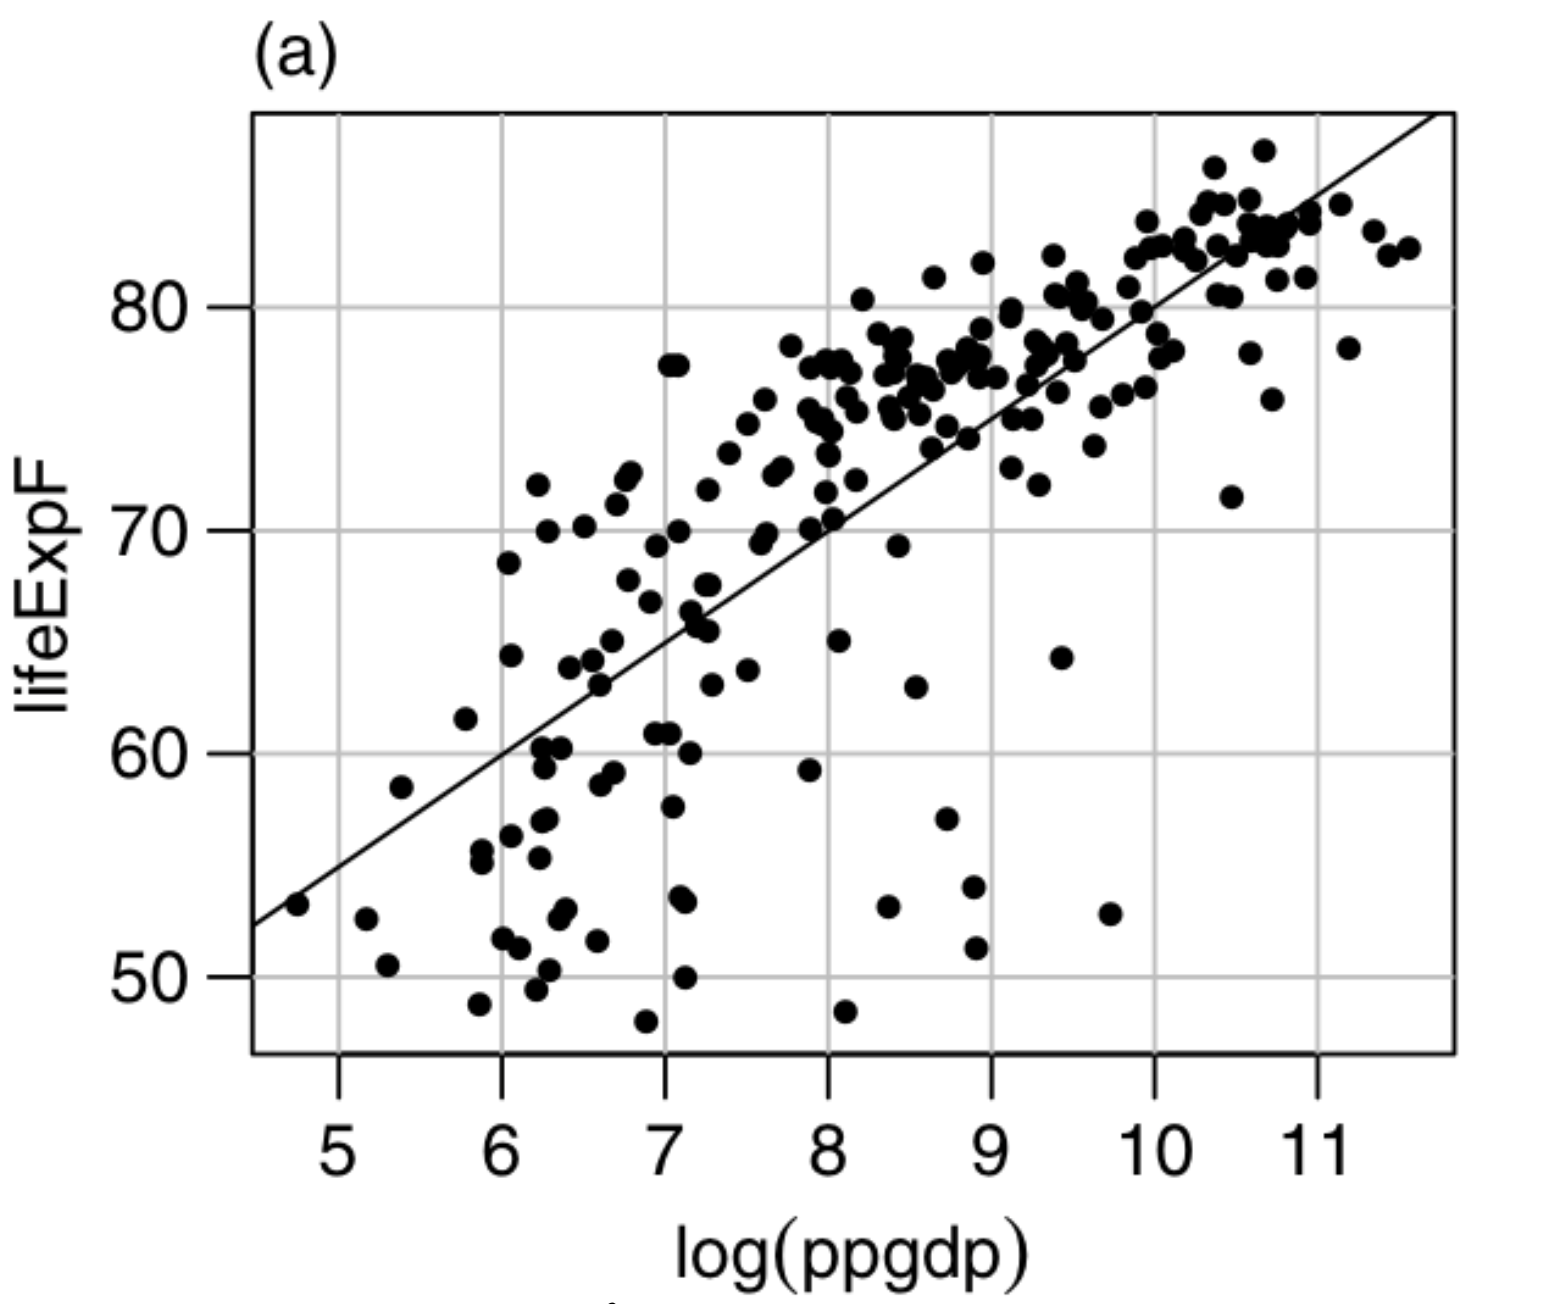
\includegraphics[width=0.55\textwidth]{fig3.png}
    \text{Extract residuals (part of lifeExpF not explained by }$\log(\text{ppgdp})$ \text{)}
\end{figure}
\noindent
2. Compute regression of fertility on $\log(\text{ppgdp})$ \textcolor{red}{-- see Fig. below}
\begin{figure}[H]
    \centering
    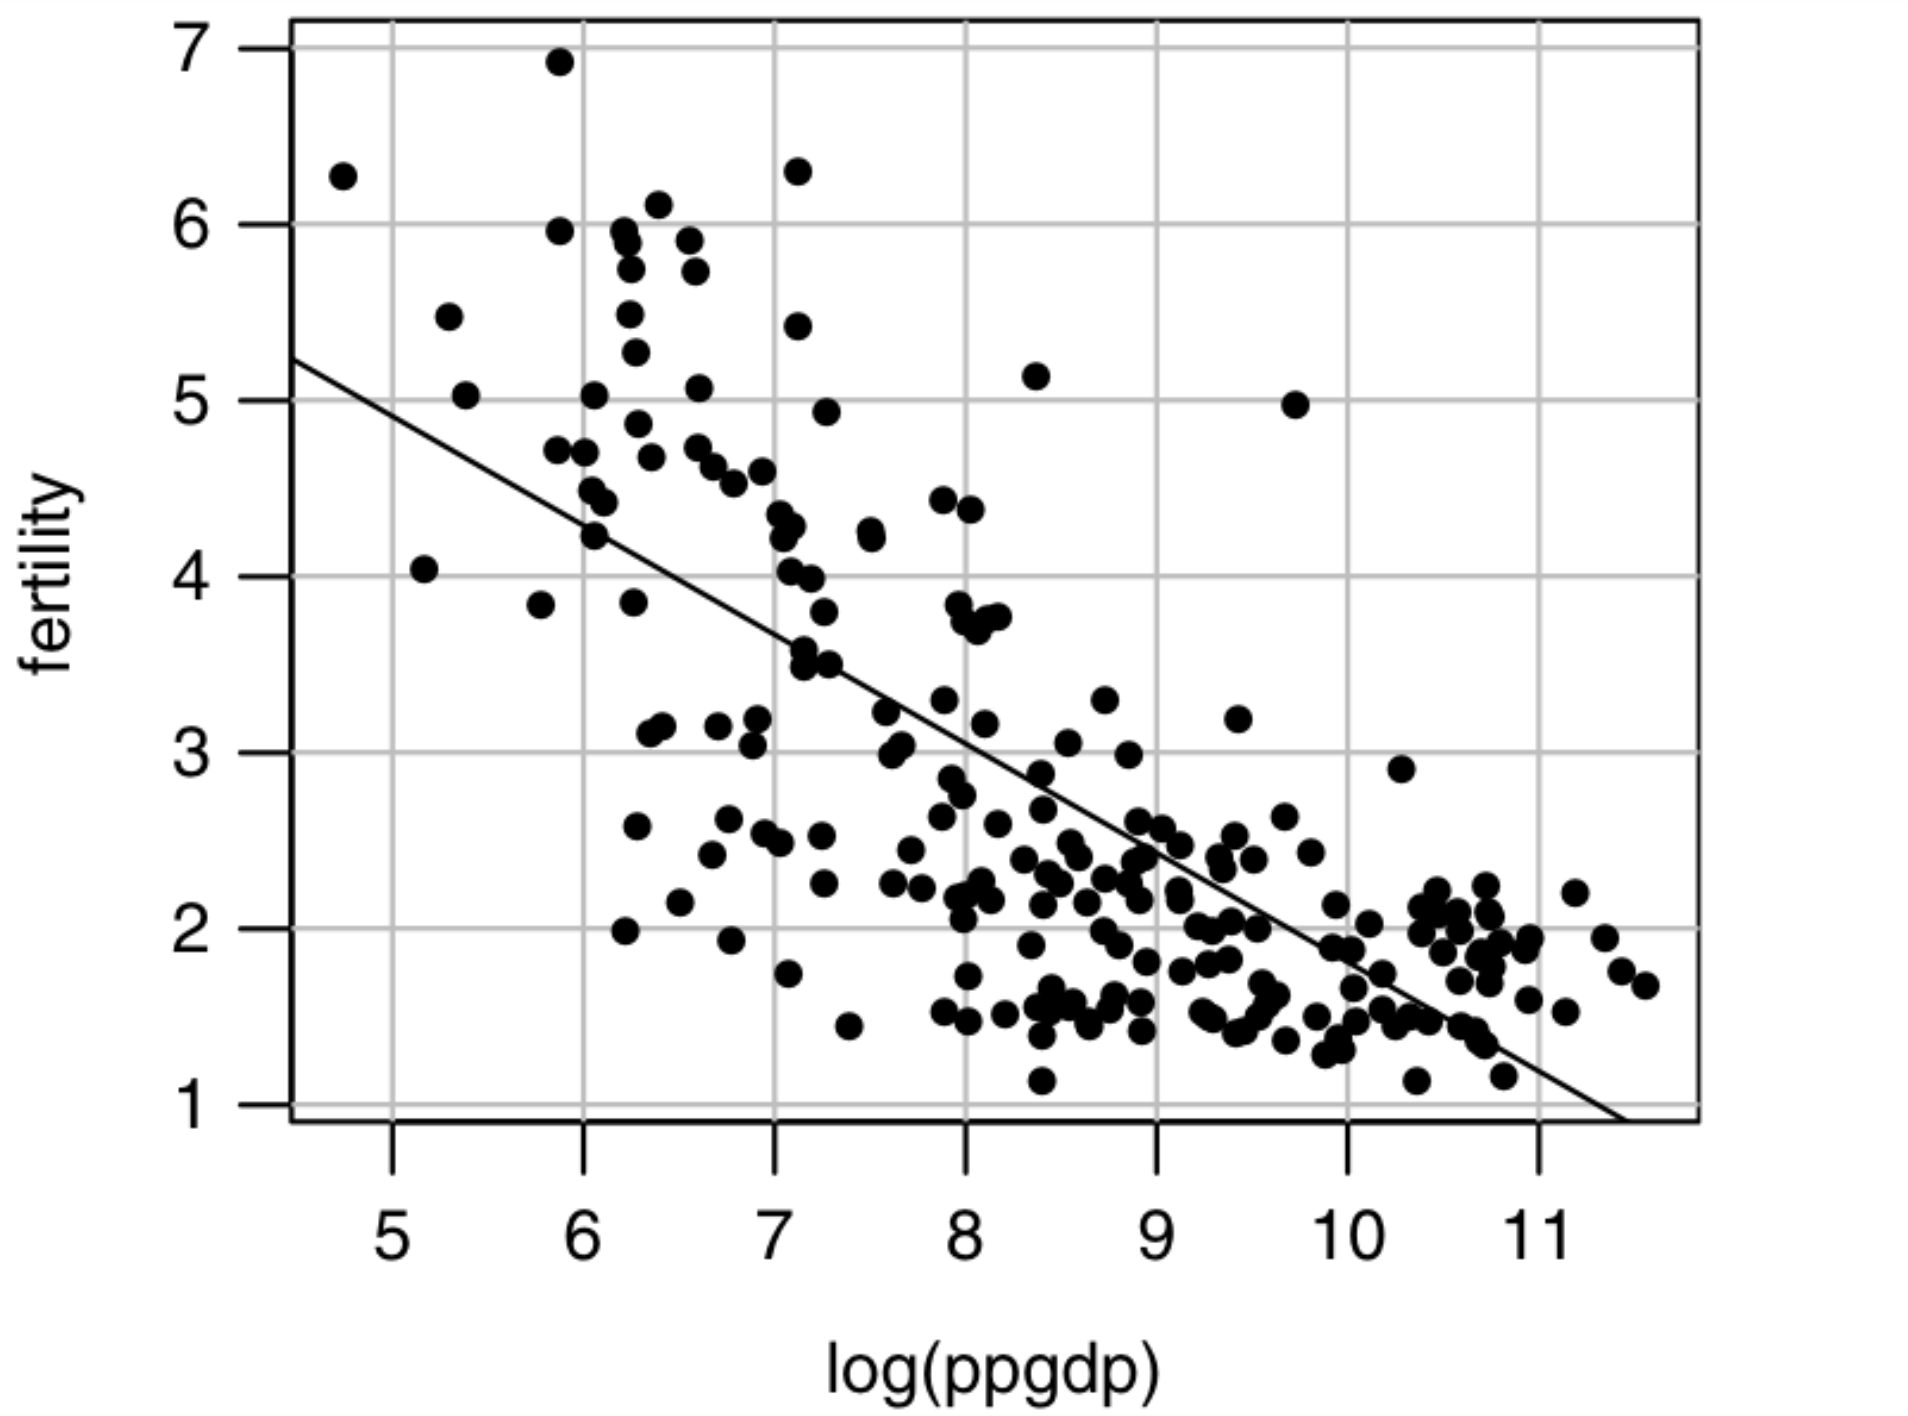
\includegraphics[width=0.55\textwidth]{fig4.png}
    \text{Extract residuals (part of fertility not explained by }$\log(\text{ppgdp})$ \text{)}
\end{figure}
\noindent
3. Plot residuals from (1) against those from (2)
\begin{figure}[H]
    \centering
    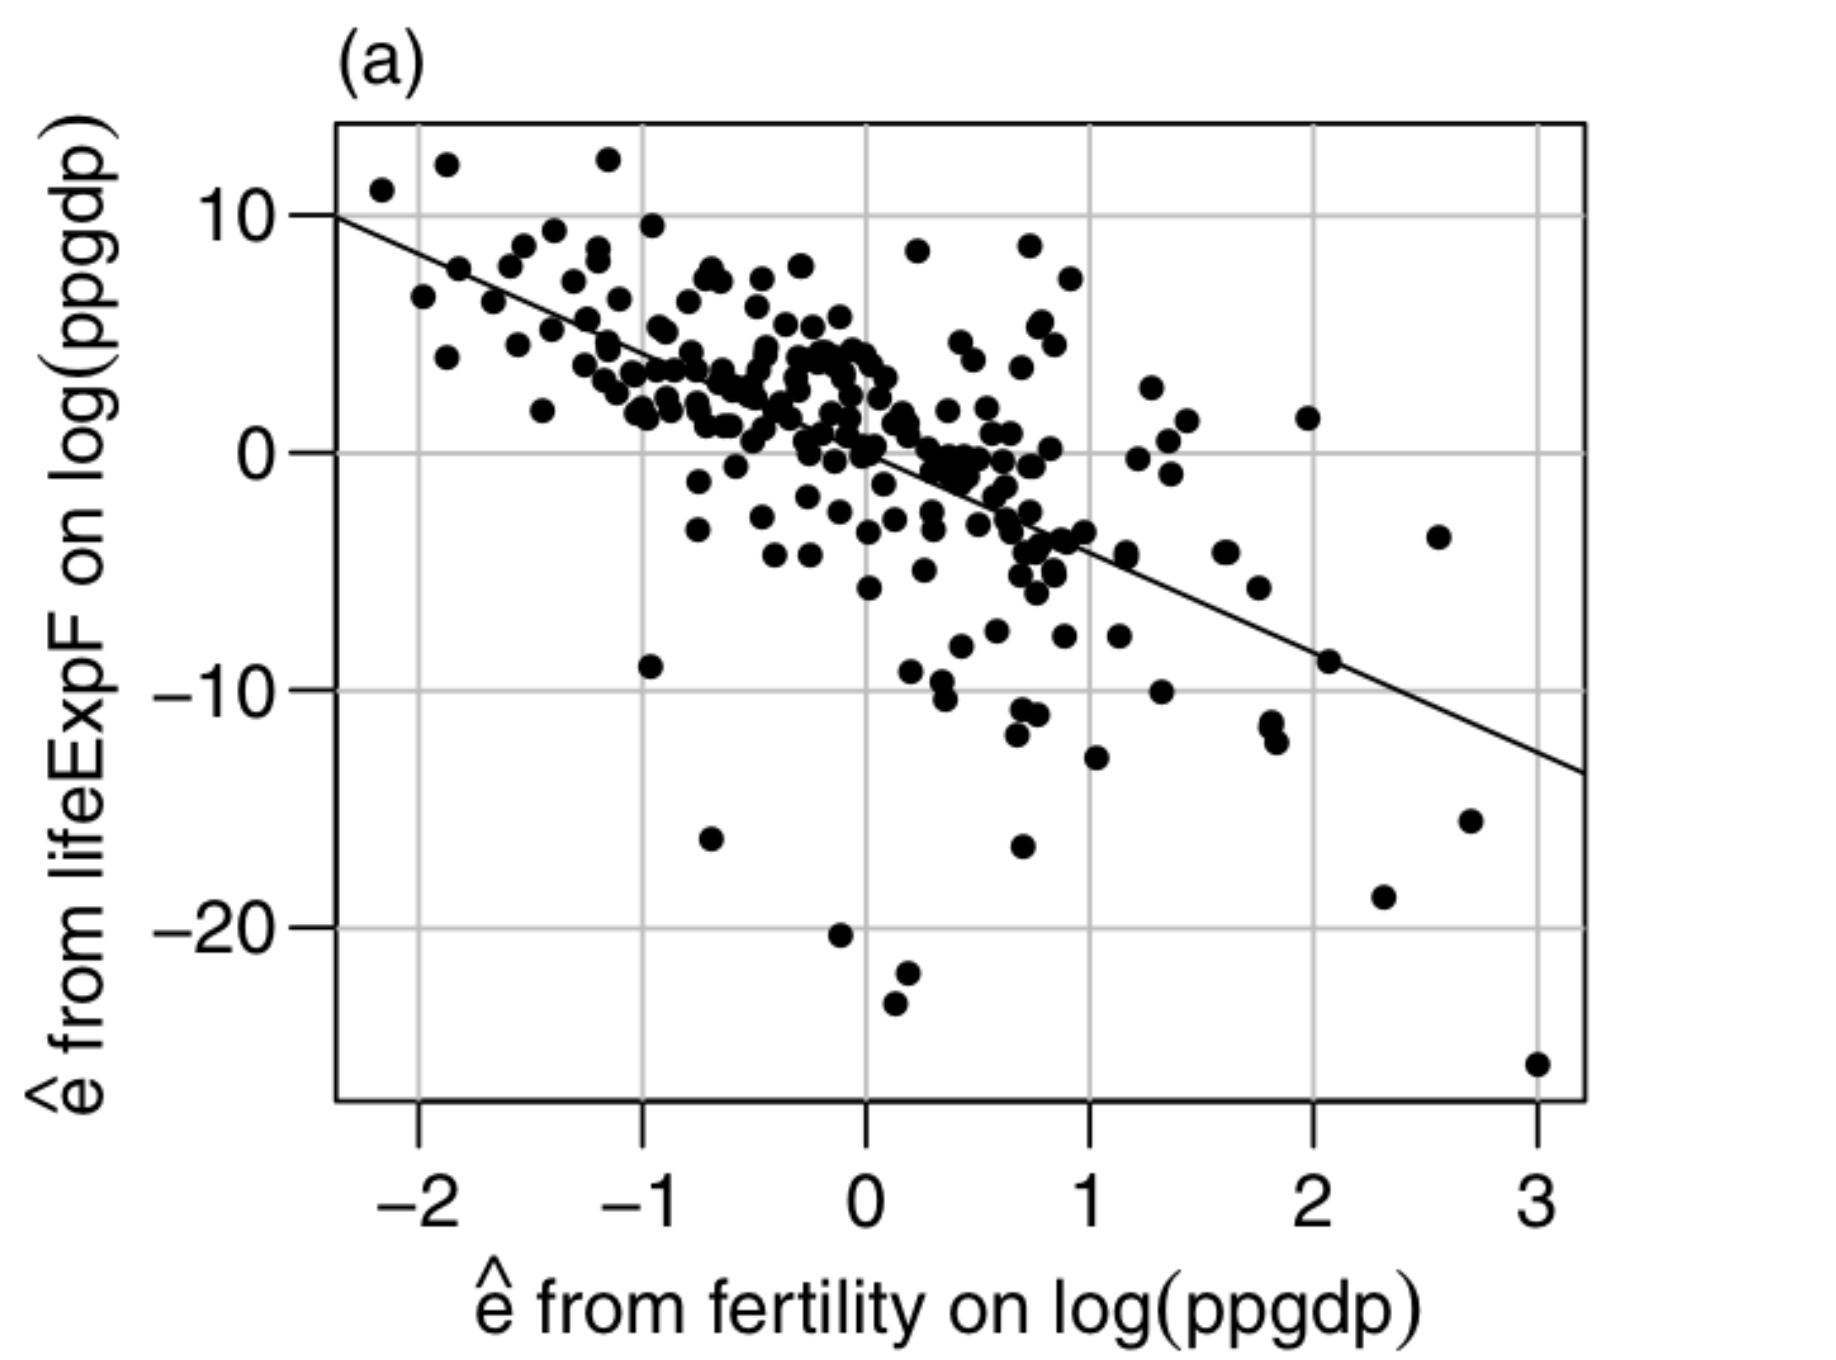
\includegraphics[width=0.55\textwidth]{fig5.png}
\end{figure}

\noindent
\textbf{Interpretation}\\
AVP summarizes the relationship between lifeExpF and fertility \textcolor{blue}{adjusting} for $\log(\text{ppgdp})$.\\
If AVP plot shows a stronger relationship than the marginal plot on fertility, then the two variables act jointly to explain extra variation.
\begin{figure}[H]
    \centering
    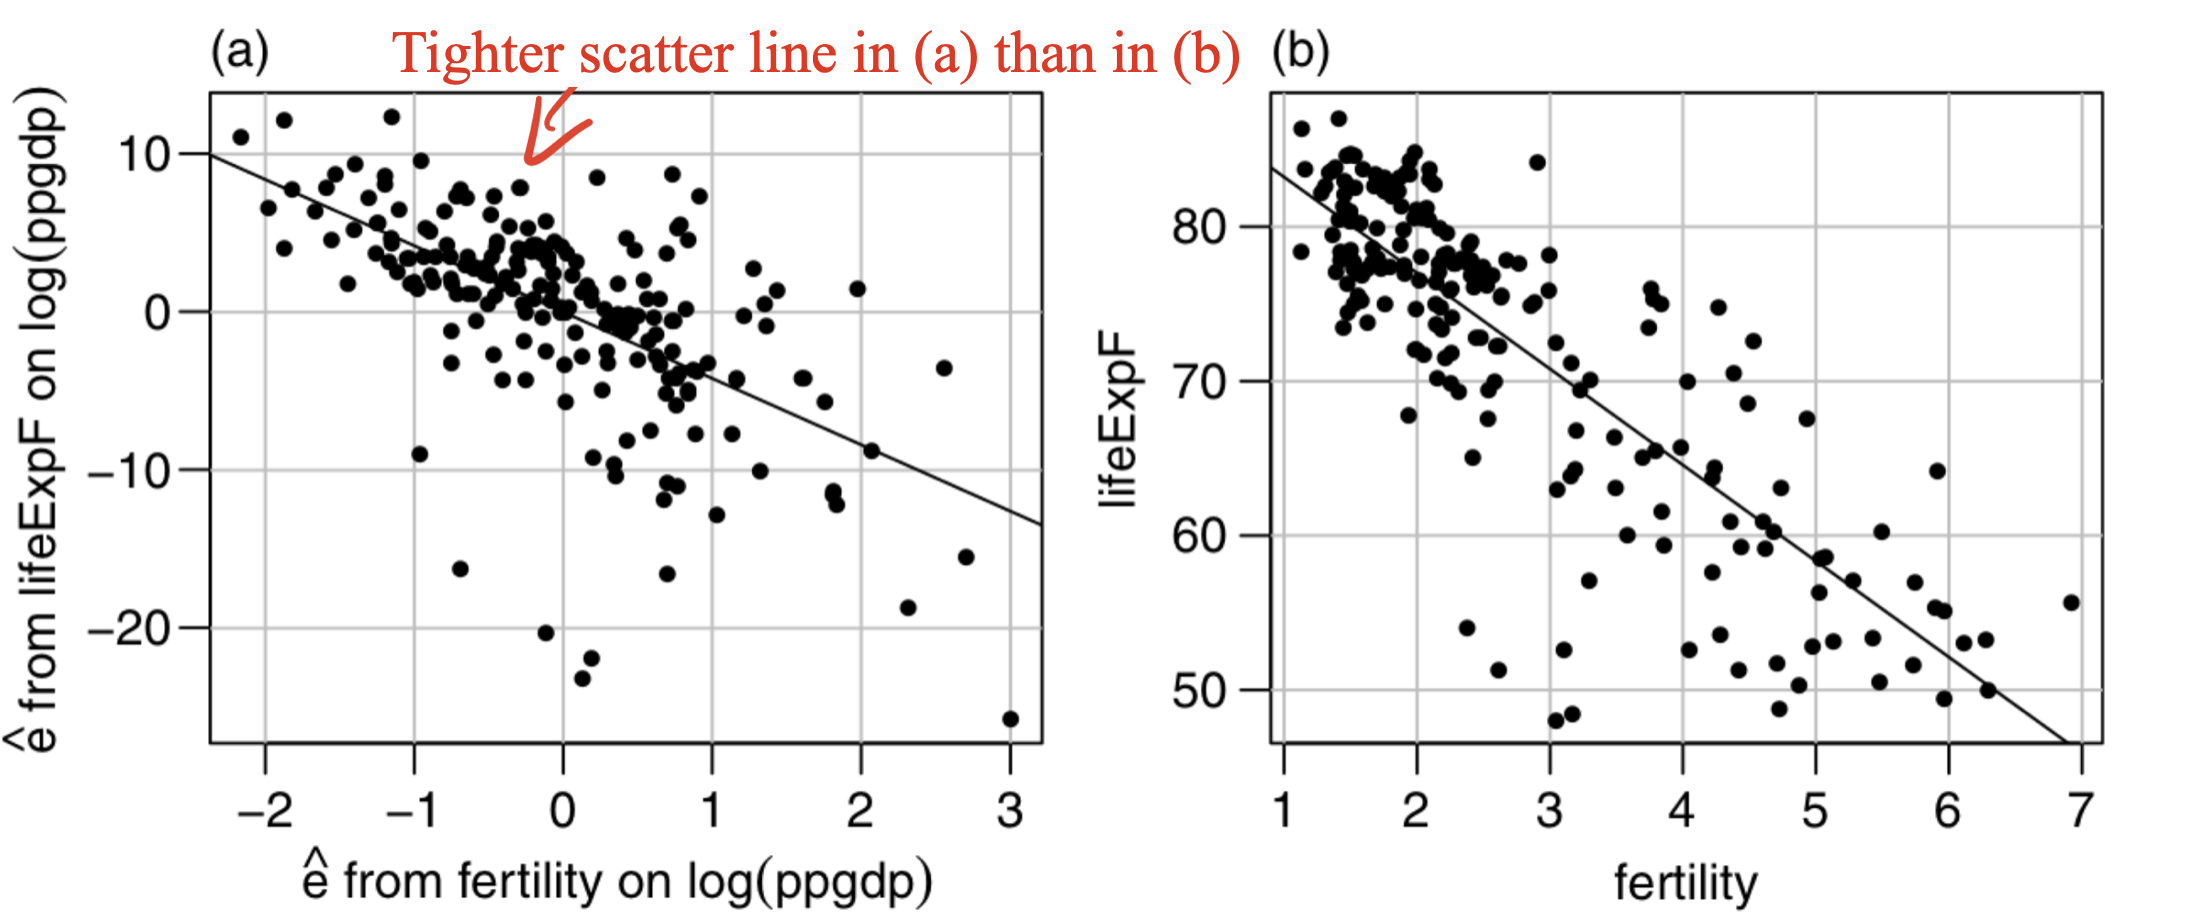
\includegraphics[width=1\textwidth]{fig6.png}
\end{figure}
\noindent
\textbf{Note:}
From AVP, when $\hat{e}$ (x-axis) = 0, $\hat{e}$ (y-axis) = 0 \textit{(intercept)}, estimated slope = $-4.199$\\
$\equiv$ Same as slope for fertility when fitting both predictors together \textit{(which we learn about next)}

\section*{Multiple Linear Regression Model}

\noindent
Assume we have response r.v. $Y$ and predictors $X_1, \dots, X_p$.
\noindent
Write
\[
E\left( Y | X \right) = \beta_0 + \beta_1 X_1 + \dots + \beta_p X_p
\]
\textcolor{blue}{\quad \quad \quad \quad \quad \quad \quad \quad (conditioning on all $X_1, \dots, X_p$)}

\noindent
With specific values $\left(x_1, \dots, x_p\right) = x$
\[
E(Y | X = x) = \beta_0 + \beta_1 x_1 + \dots + \beta_p x_p
\]
\noindent
\textcolor{red}{$\beta_0 \dots \beta_p$ unknown parameters to be estimated from sample of data}

\section*{Fuel Consumption Data}
\begin{figure}[H]
    \centering
    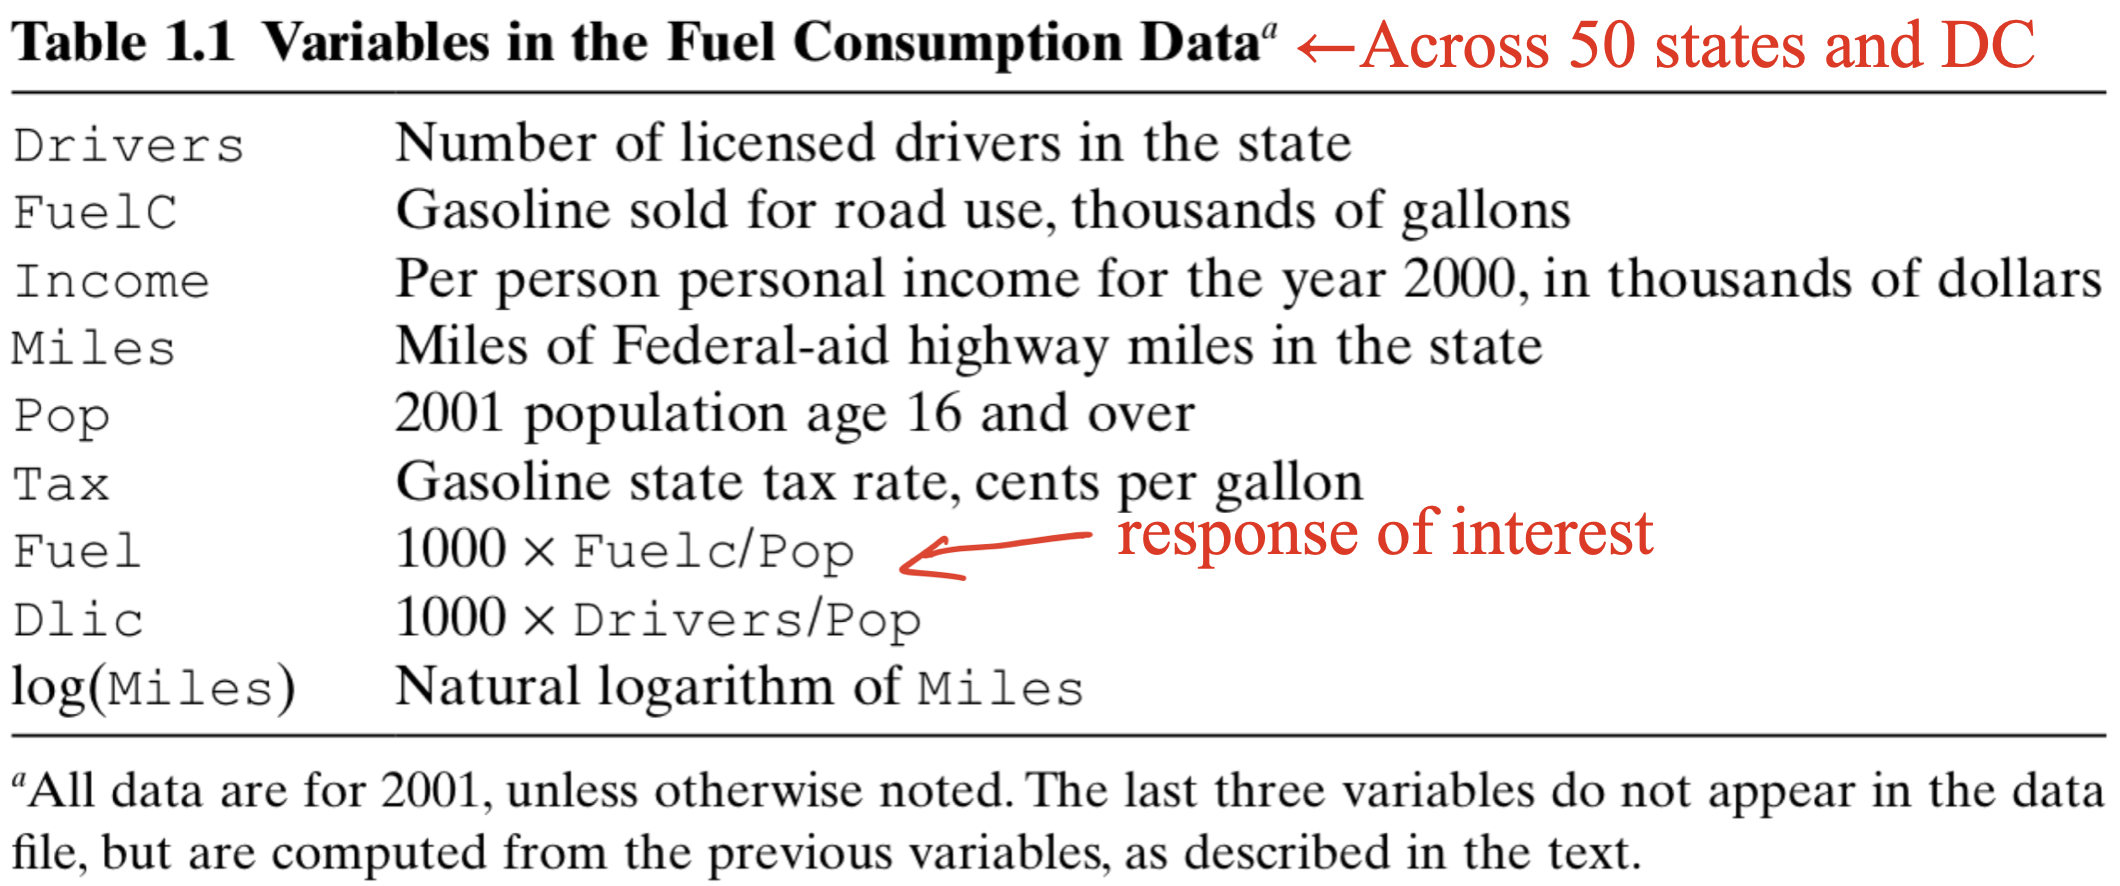
\includegraphics[width=1\textwidth]{fig7.png}
\end{figure}
\begin{figure}[H]
    \centering
    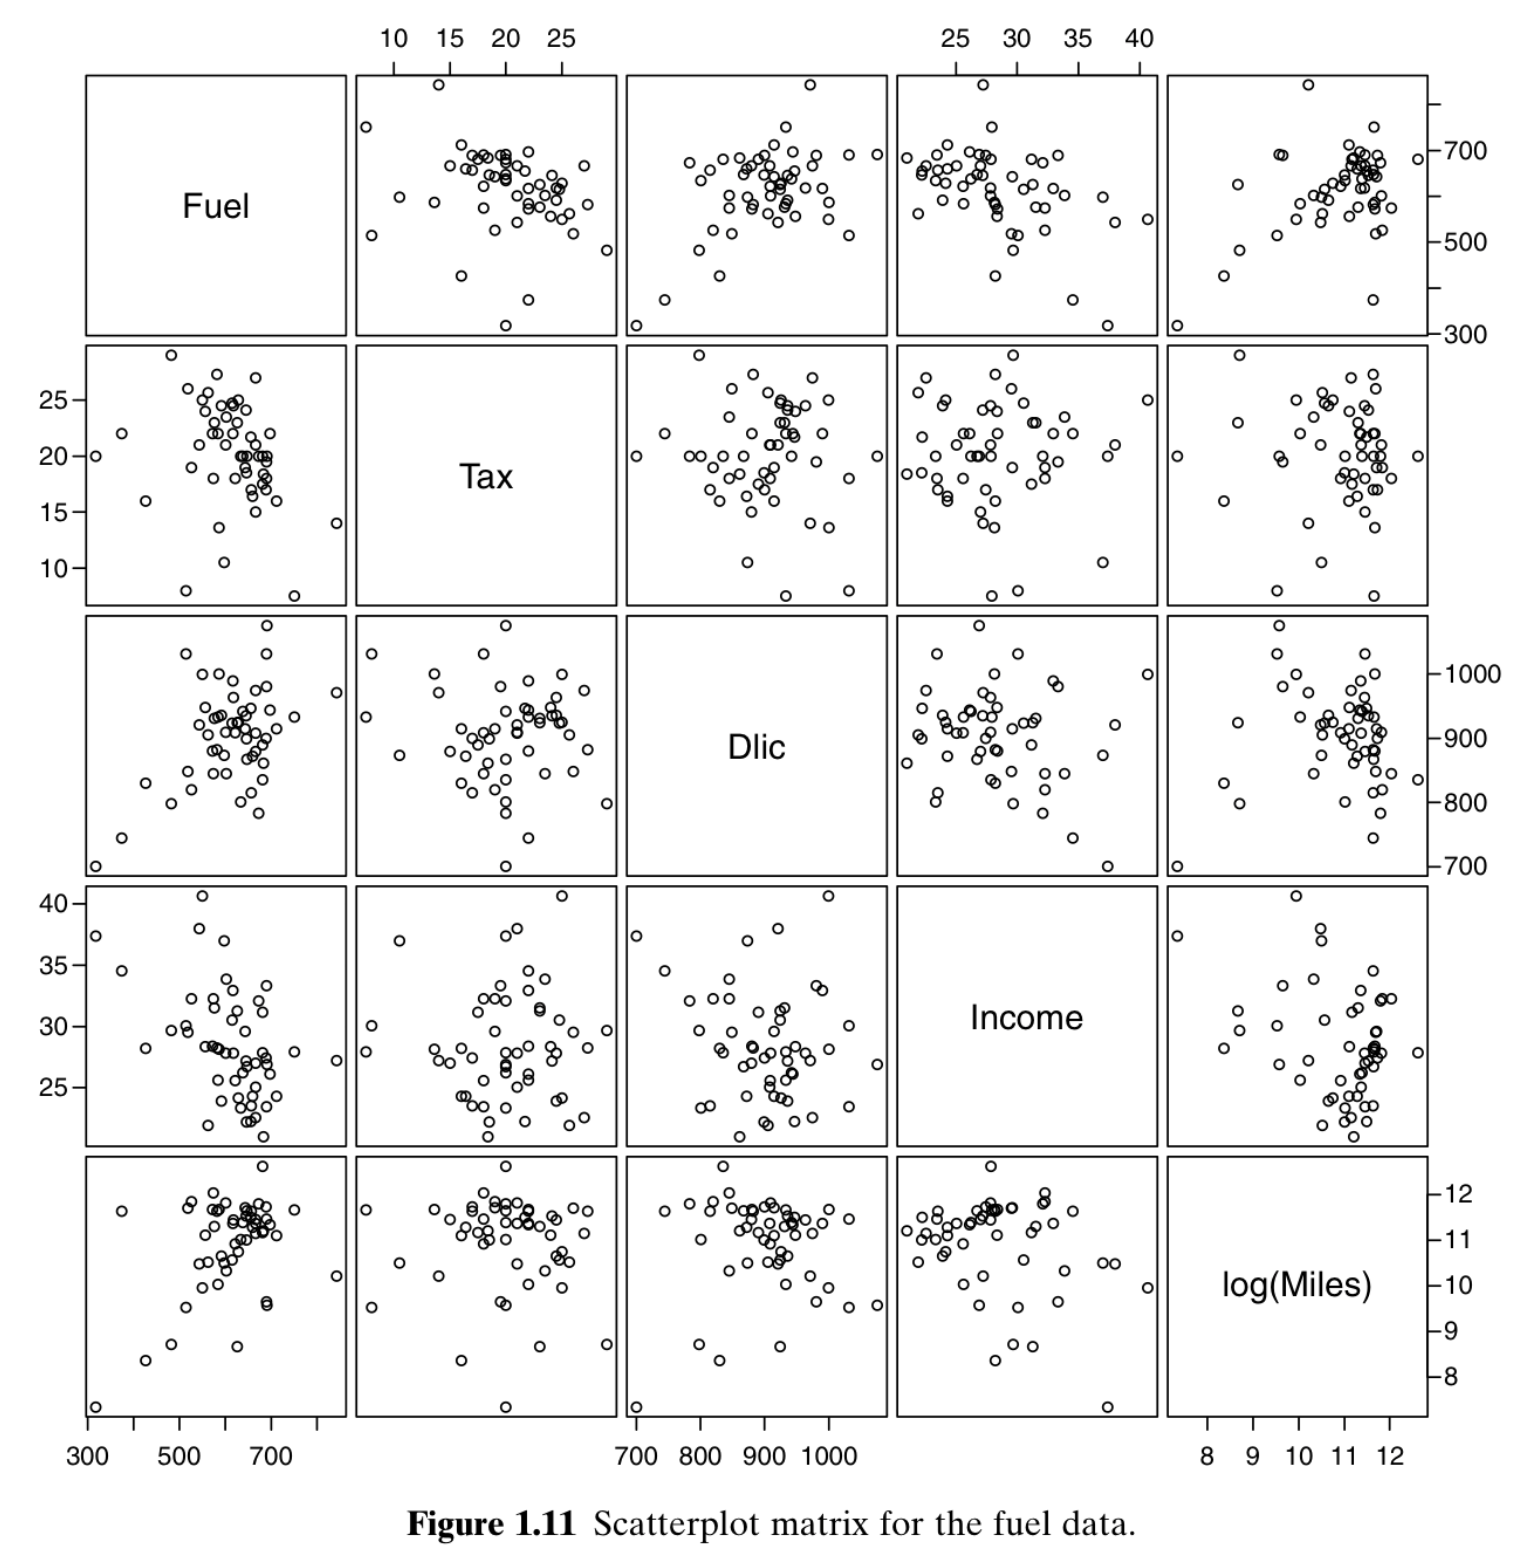
\includegraphics[width=1\textwidth]{fig8.png}
\end{figure}

\textbf{Table 3.1 Summary Statistics for the Fuel Data}\\
\begin{tabularx}{\textwidth}{l r r r r r}
\hline
 & \textbf{N} & \textbf{Average} & \textbf{Std Dev} & \textbf{Min} & \textbf{Max} \\
\hline
Tax       & \quad \quad 51 & \quad \quad \quad 20.15 & \quad \quad \quad 4.54 & \quad \quad \quad 7.50  & \quad \quad \quad 29.00 \\
Dlic      & 51 & 903.68 & 72.86 & 700.20 & 1075.29 \\
Income    & 51 & 28.40 & 4.45 & 20.99  & 40.64 \\
log(Miles)& 51 & 10.91 & 1.03 & 7.34   & 12.61 \\
Fuel      & 51 & 613.13 & 88.96 & 317.49 & 842.79 \\
\hline
\end{tabularx}

\bigskip

\textbf{Table 3.2 Sample Correlations for the Fuel Data}\\
\begin{tabularx}{\textwidth}{l r r r r r}
\hline
 & \textbf{Tax} & \textbf{Dlic} & \textbf{Income} & \textbf{log(Miles)} & \textbf{Fuel} \\
\hline
\textbf{Tax}       & \quad 1.0000 & \quad -0.0858 & \quad -0.0107 & \quad -0.0437 & \quad -0.2594 \\
\textbf{Dlic}      & -0.0858 & 1.0000 & -0.1760 & 0.0306  & 0.4685  \\
\textbf{Income}    & -0.0107 & -0.1760 & 1.0000 & -0.2959 & -0.4644 \\
\textbf{log(Miles)}& -0.0437 & 0.0306  & -0.2959 & 1.0000  & 0.4220  \\
\textbf{Fuel}      & -0.2594 & 0.4685  & -0.4644 & 0.4220  & 1.0000  \\
\hline
\end{tabularx}

\section*{Data and Matrix Notation}
\[
\mathbf{Y} =
\begin{pmatrix}
y_1 \\
y_2 \\
\vdots \\
y_n
\end{pmatrix}
\quad
\mathbf{X} =
\begin{pmatrix}
1 & x_{11} & \dots & x_{1p} \\
1 & x_{21} & \dots & x_{2p} \\
\vdots & \vdots & \ddots & \vdots \\
1 & x_{n1} & \dots & x_{np}
\end{pmatrix}
\]
\noindent
\textbf{For fuel consumption dataset,}
\[
\mathbf{X} = 
\begin{pmatrix}
1 & 18.00 & 1031.38 & 23.471 & 16.5271 \\
1 & 8.00  & 1031.64 & 30.064 & 13.7343 \\
1 & 18.00 & 908.597 & 25.578 & 15.7536 \\
\vdots & \vdots & \vdots & \vdots & \vdots \\
1 & 25.65 & 904.894 & 21.915 & 15.1751 \\
1 & 27.30 & 882.329 & 28.232 & 16.7817 \\
1 & 14.00 & 970.753 & 27.230 & 14.7362
\end{pmatrix}
\quad
\mathbf{Y} = 
\begin{pmatrix}
690.264 \\
514.279 \\
621.475 \\
\vdots \\
562.411 \\
581.794 \\
842.792
\end{pmatrix}
\]
\noindent
\textbf{Now define MLR model :}
\[
E(Y | X = x_i) = \beta_0 + \beta_1 x_{i1} + \dots + \beta_p x_{ip} = x_i' \beta
\]
\noindent
\textcolor{red}{This is the mean function evaluated at $x_i$.}\\
\noindent
The mean function across all $n$ observations is
\[
E(Y_{\textcolor{red}{n \times 1}} | X_{\textcolor{red}{n \times (p+1)}}) = X_{\textcolor{red}{n \times (p+1)}} \beta_{\textcolor{red}{(p+1) \times 1}}
\textcolor{blue}{\quad (p+1 \text{ allows for intercept})}
\]


\section*{What about the errors in the model?}

\noindent
Define elementwise
\[
e_i = y_i - E(Y | X = x_i) = y_i - x_i' \beta
\]
\noindent
and note
\[
e = \begin{pmatrix} e_1, \dots, e_n \end{pmatrix}'
\]
\noindent
We assume
\[
\left.
\begin{array}{c}
E(e | X) = 0_{\textcolor{red}{n \times 1}}\\
\text{var}(e | X) = \sigma^2 I_{\textcolor{red}{n \times n}}    
\end{array}
\right]
\textcolor{blue}{\text{Key Assumptions}}
\]
\textcolor{blue}{\quad \quad \quad \quad \text{I: independence of errors and constant variance}}

\noindent
The adjective \textcolor{red}{linear} means the model is linear in its parameters $\beta_0, \dots, \beta_p$.

\noindent
Examples:
\[
\textcolor{blue}{Y = \beta_0 + \beta_1 X + \beta_2 X^2 + e}
\]
\[
\textcolor{blue}{Y = \beta_0 + \beta_1 \log(X) + e}
\]
\noindent
\textcolor{red}{Models are written out as a function of the r.v.'s $X$ and $Y$.}\\
\textcolor{red}{Both models are linear even though the relationship between $Y$ and $X$ is not linear.}

\noindent
\textbf{Some non-linear models can be turned linear.}\\
\textcolor{blue}{Example:\\Non-linear model:
\[
E(Y | X) = \frac{X}{\alpha X + \beta}
\]}
\noindent
\textcolor{blue}{Take reciprocal:
\[
E\left(\frac{1}{Y} \Big| X\right) = \alpha + \beta \left(\frac{1}{X}\right)
\]}
\textcolor{red}{
\[
Y' = \frac{1}{Y}, \quad X' = \frac{1}{X}
\]
\[
\Rightarrow E(Y' | X') = \alpha + \beta X
\]}

\noindent
\textcolor{blue}{\textbf{Another Example}\\
Volume of trees $\approx c r^2 h$\\
or more generally
\[
\alpha r^{\beta_1} h^{\beta_2}
\]}
\noindent
\textcolor{blue}{$\Rightarrow$ Non-linear model:
\[
E(\text{vol} | r, h) = \alpha r^{\beta_1} h^{\beta_2}
\]}
\noindent
\textcolor{blue}{Take logarithm:}
\[
\underbrace{E(\log(\text{vol}) | r, h)}_{\textcolor{red}{Y}} = \underbrace{\log(\alpha)}_{\textcolor{red}{\beta_0}} + \underbrace{\beta_1 \log(r)}_{\textcolor{red}{x_1}} + \underbrace{\beta_2 \log(h)}_{\textcolor{red}{x_2}}
\]

\noindent
\textbf{Which of the following models are linear?}

\begin{itemize}
  \item[(a)] $Y = \beta_0 + \beta_1^{X_1} + \varepsilon$
  \item[(b)] $Y = \beta_0 \beta_1^{X_1} \varepsilon$
  \item[(c)] $Y = \beta_0 + \beta_1 e^X + \varepsilon$ \dotfill \textcolor{orange}{Linear}
  \item[(d)] $Y = \beta_0 + \beta_1 X^2 + \beta_2 \log(X) + \varepsilon$ \dotfill \textcolor{orange}{Linear}
\end{itemize}

\bigskip

\noindent
\textbf{Which below can be turned linear after transformation?}

\begin{itemize}
  \item[(a)] $Y = \beta_0 + \beta_1^{X_1} + \varepsilon$
  \item[(b)] $Y = \beta_0 \beta_1^{X_1} \varepsilon$
\end{itemize}

\textbf{Ans: (b)}

\section*{Ordinary Least Square Estimators}
\begin{figure}[H]
    \centering
    \begin{minipage}{0.5\textwidth}
        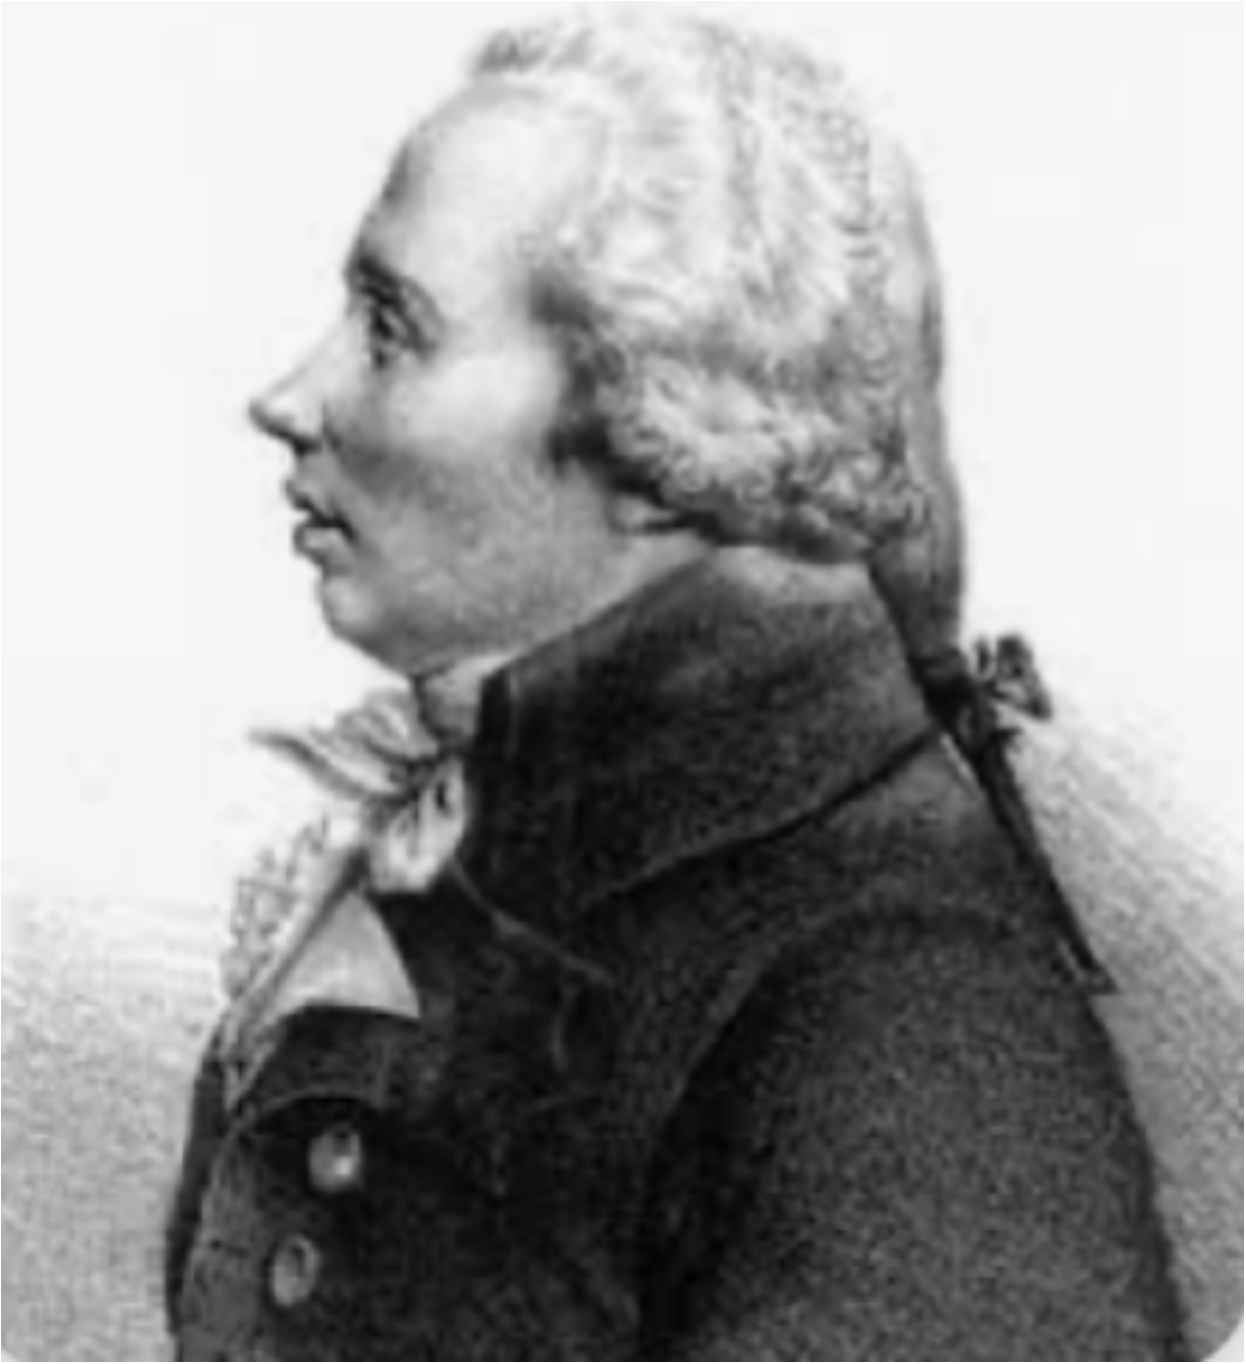
\includegraphics[width=\textwidth]{fig9.png}
    \end{minipage}%
    \hfill
    \begin{minipage}{0.5\textwidth}
        \vspace*{0.01\textheight} % Adjust the vertical position of the text
        \centering
        \textbf{Legendre}
    \end{minipage}
\end{figure}

\begin{figure}[H]
    \centering
    \begin{minipage}{0.5\textwidth}
        \vspace*{0.01\textheight}
        \raggedright 
        Recall for SLR, the least squares estimate $(\hat{\beta}_0, \hat{\beta}_1)$ for $(\beta_0, \beta_1)$ is the intercept and slope of the straight line with the minimum sum of squared vertical distances to the data points
        \[
        \sum_{i=1}^{n} (y_i - \hat{\beta}_0 - \hat{\beta}_1 x_i)^2.
        \]
    \end{minipage}
    \hfill
    \begin{minipage}{0.45\textwidth}
        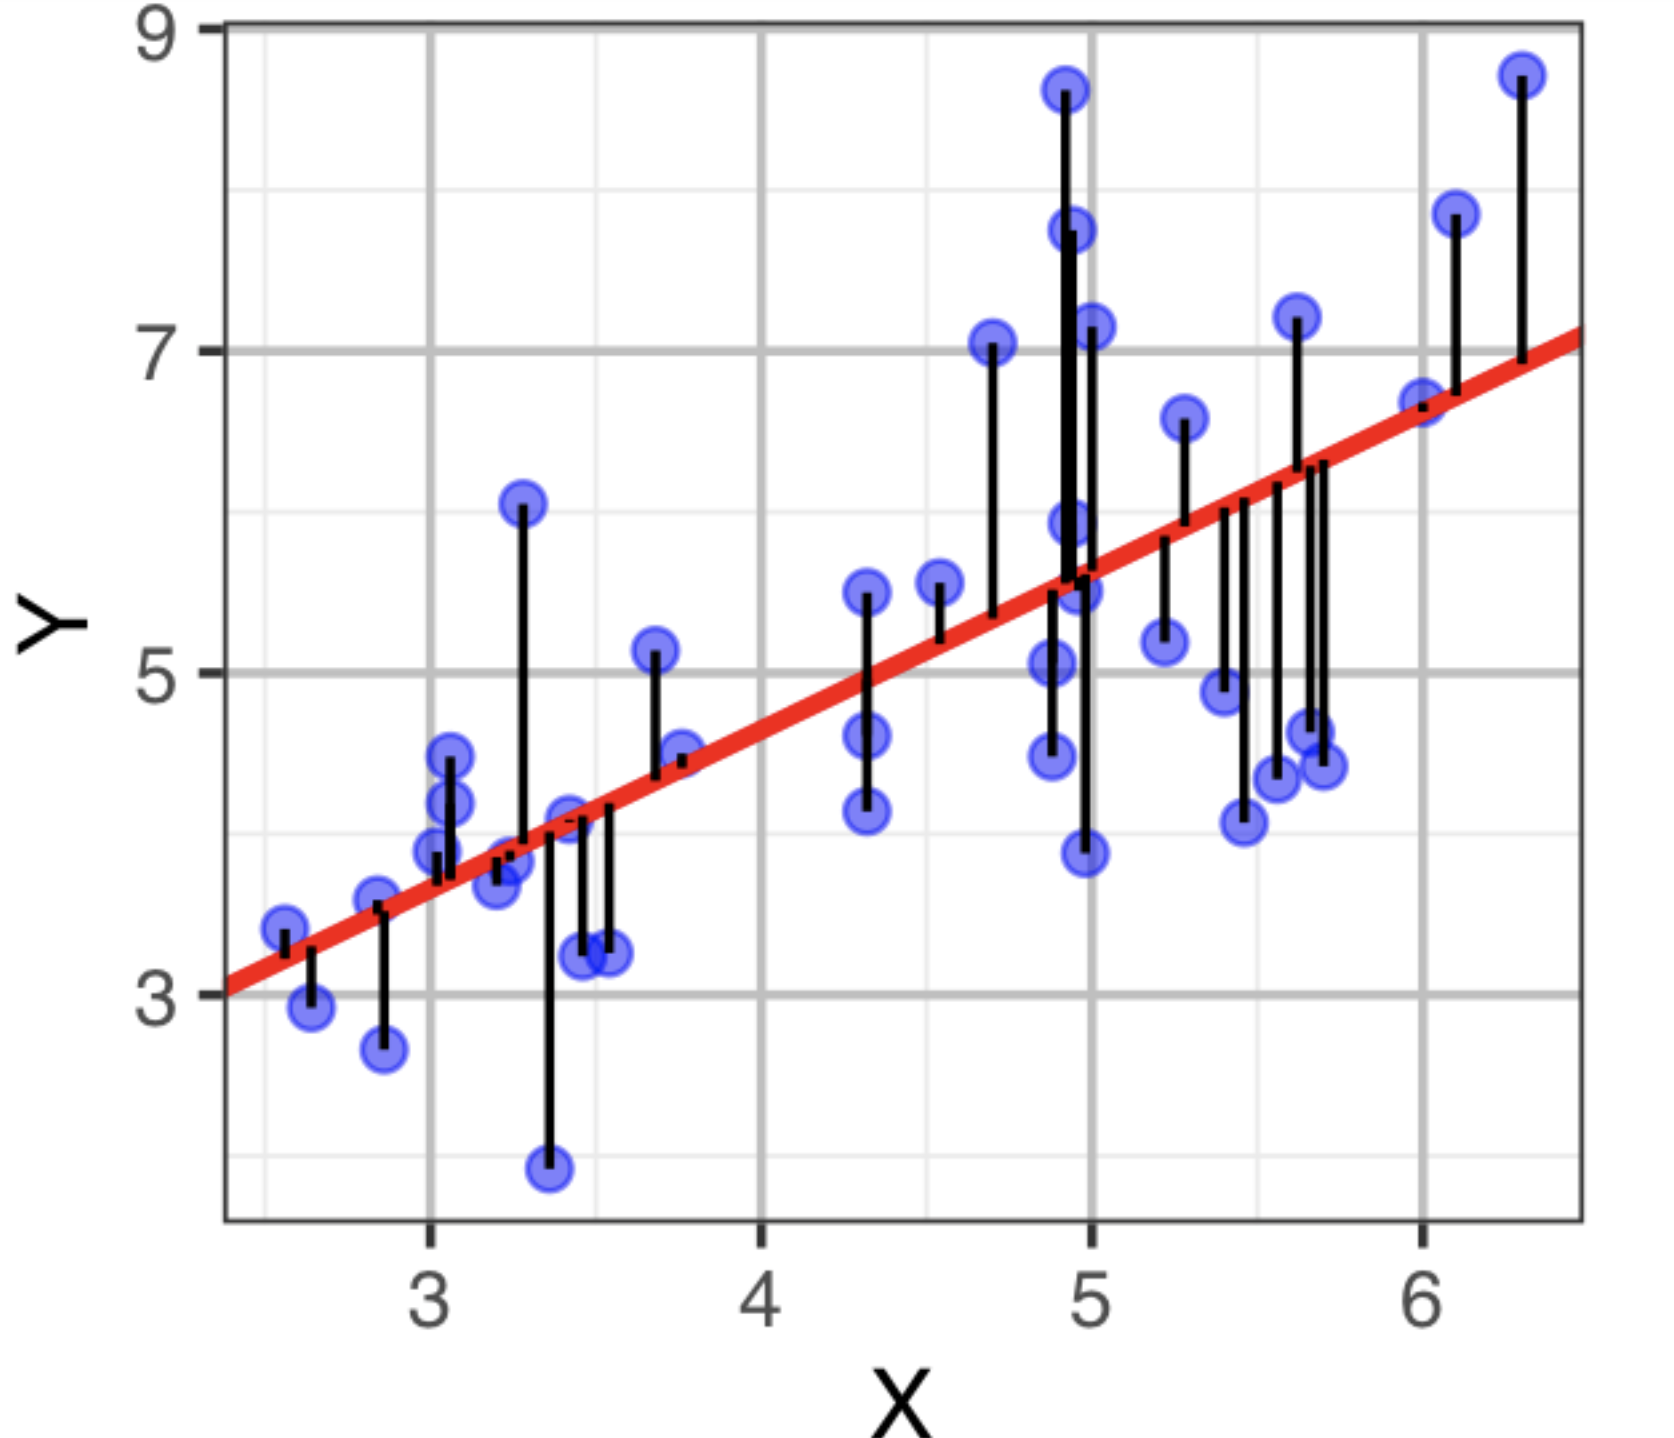
\includegraphics[width=\textwidth]{fig10.png}
    \end{minipage}
\end{figure}

\noindent
MLR is just like SLR. The least squares estimate $(\hat{\beta}_0, \dots, \hat{\beta}_p)$ for $(\beta_0, \dots, \beta_p)$ is the intercept and slopes of the (hyper)plane with the minimum sum of squared vertical distance to the data points
\[
\sum_{i=1}^{n} (y_i - \hat{\beta}_0 - \hat{\beta}_1 x_{i1} - \dots - \hat{\beta}_p x_{ip})^2.
\]

\noindent
To find $(\hat{\beta}_0, \hat{\beta}_1, \dots, \hat{\beta}_p)$ minimize
\[
\text{RSS}(\beta_0, \beta_1, \dots, \beta_p)
= L(\beta_0, \beta_1, \dots, \beta_p)
= \sum_{i=1}^{n} e_i^2\]
\[
= \sum_{i=1}^{n} (y_i - \beta_0 - \beta_1 x_{i1} - \dots - \beta_p x_{ip})^2
\]
\noindent
\textcolor{red}{Take partial derivatives and equate to 0}
\[
\frac{\partial L}{\partial \beta_0} = -2 \sum_{i=1}^{n} (y_i - \beta_0 - \beta_1 x_{i1} - \dots - \beta_p x_{ip})
\]
\[
\frac{\partial L}{\partial \beta_k} = -2 \sum_{i=1}^{n} x_{ik} (y_i - \beta_0 - \beta_1 x_{i1} - \dots - \beta_p x_{ip})
\text{ for } k = 1, 2, \dots, p
\]

\noindent
OLS estimates are the solution to the following system of equations, called \textcolor{blue}{normal equations}:
\[
\begin{aligned}
\beta_0 \textcolor{red}{n} &+ \beta_1 \textcolor{red}{\sum_{i=1}^{n} x_{i1}} + \dots + \beta_p \textcolor{red}{\sum_{i=1}^{n} x_{ip}} = \textcolor{red}{\sum_{i=1}^{n} y_i} \\
\beta_0 \textcolor{red}{\sum_{i=1}^{n} x_{i1}} &+ \beta_1 \textcolor{red}{\sum_{i=1}^{n} x_{i1}^2} + \dots + \beta_p \textcolor{red}{\sum_{i=1}^{n} x_{i1} x_{ip}} = \textcolor{red}{\sum_{i=1}^{n} x_{i1} y_i} \\
&\vdots \\
\beta_0 \textcolor{red}{\sum_{i=1}^{n} x_{ik}} &+ \beta_1 \textcolor{red}{\sum_{i=1}^{n} x_{i1} x_{ik}} + \dots + \beta_p \textcolor{red}{\sum_{i=1}^{n} x_{ik} x_{ip}} = \textcolor{red}{\sum_{i=1}^{n} x_{ik} y_i} \\
&\vdots \\
\beta_0 \underbrace{\textcolor{red}{\sum_{i=1}^{n} x_{ip}}}_{\textcolor{blue}{known}} &+ \beta_1 \underbrace{\textcolor{red}{\sum_{i=1}^{n} x_{ip} x_{i1}}}_{\textcolor{blue}{known}} + \dots + \beta_p \underbrace{\textcolor{red}{\sum_{i=1}^{n} x_{ip}^2}}_{\textcolor{blue}{known}} = \underbrace{\textcolor{red}{\sum_{i=1}^{n} x_{ip} y_i}}_{\textcolor{blue}{known}}
\end{aligned}
\]

\noindent
Usually, we write this in matrix form:
\[
\text{RSS}(\beta) = \sum_{i=1}^{n} e_i^2 = (Y_{\textcolor{red}{n \times 1}} - X\beta_{\textcolor{red}{n \times 1}})'(Y - X\beta)
{\textcolor{red}{\text{(matrix notation of observables)}}}
\]
Using the distributive property for matrices:
\[
\text{RSS}(\beta) = Y'Y + \beta'(X'X)\beta - 2Y'X\beta
\]
Differentiate with respect to $\beta$ and set to 0 to solve the \textcolor{blue}{normal equations}:
\[
\Rightarrow X'X \beta = X'Y
\]
\[
\Rightarrow \hat{\beta} = (X'X)^{-1}X'y
\]
\noindent
Let's look more closely at how normal equations arise:
\[
\frac{\partial RSS(\beta)}{\partial \beta} = -2X'(\underbrace{Y - X\beta}_{\textcolor{red}{e}}) = 0
\]
\[
\Rightarrow X'X\beta= X'Y
\]
\textcolor{blue}{What is this saying?} \\
\textcolor{blue}{That the solution to $\beta$ will produce $\hat{e} = (Y - X\hat{\beta})$} 
\textcolor{blue}{that are orthogonal to the column space of $X$.}

\newpage 
\section*{Properties of OLS estimators}
\noindent
\textcolor{blue}{Under Key Assumptions:}
\[
E(\hat{\beta} | X) = E[(X'X)^{-1}X'Y | X]
\]
\[
= [(X'X)^{-1}X']E(Y | X)
\]
\[
= (X'X)^{-1}X'X\beta
\]
\[
= \beta
\]
\noindent
$\therefore \hat{\beta}$ is unbiased for $\beta$ if the model is true.
\[
\text{Var}(\hat{\beta} | X) = \text{Var}[(X'X)^{-1}X'Y | X]
\]
\[
= (X'X)^{-1}X'[\text{Var}(Y | X)]X(X'X)^{-1}
\]
\[
= (X'X)^{-1}X'[\sigma^2 I]X(X'X)^{-1}
\]
\[
= \sigma^2 (X'X)^{-1}
\]

\subsection*{Gauss-Markov Theorem}

\noindent
Under key assumptions, OLS estimator is \textcolor{blue}{efficient} in the class of linear unbiased estimators. \\
i.e., for any unbiased estimator $b$ that is linear in $Y$, 
\[
\text{Var}(b | X) \geq \text{Var}(\hat{\beta} | X)
\]
\textbf{Sketch of Proof}\\
Since \( b \) is assumed linear in \( Y \), \\
we can write it as
\[b = C Y  \text{for some matrix } C.
\]
Let 
\[
 D = C - A  \quad \text{or} \quad C = D + A \quad \text{where} \quad A = (X' X)^{-1} X'
\]
Then,
\[
b = (D + A)Y
\]
\[
= DY + AY
\]
\[
= D(Xb + e) + \hat{\beta}
\]
(since \( Y = X\beta + e \) and \( AY = (X'X)^{-1}X'Y = \hat{\beta} \))
\[
= DXb + De + \hat{\beta}
\]
\[
E(b | X) = DXb + E(De | X) + E(\hat{\beta} | X)
\]
Since both \(b\) and \(\hat{\beta}\) are unbiased and since
\[
E(De | X) = D E(e | X) = 0
\]
\[
\Rightarrow DXb = 0
\]
\[
\therefore b = De + \hat{\beta} \text{ and } b - \beta = De + (b - \beta) = (D + A) e
\]
\[
\therefore \text{Var}(b | X) = \text{Var}(b - \beta | X) = \text{Var}((D + A)e | X)
\]
\[
= (D + A) \text{Var}(e | X) (D' + A')
\]
\[
= \sigma^2 (D + A)(D' + A') \quad \text{since Var}(e | X) = \sigma^2 I
\]
\[
= \sigma^2 (DD' + AD' + DA' + AA')
\]
\[
\text{But } DA' = D X (X'X)^{-1} = 0 \quad \text{since } DX = 0
\]
\[
\text{Also } AA' = (X'X)^{-1}
\]
\[
\therefore \text{Var}(b | X) = \sigma^2 (DD' + (X'X)^{-1}) \geq \sigma^2 (X'X)^{-1}
\]
\[
\text{Since } D'D \text{ is positive semi-definite.}
\]
\begin{table}[H]
\centering
\begin{tabular}{|l|l|}
\hline
\textbf{With fixed }$x$ & \textbf{With random }$x$ \\ \hline
SR1: $y = \beta_1 + \beta_2 x + e$ with $x$ fixed & A10.1: $y = \beta_1 + \beta_2 x + e$ with $x, y, e$ random \\ \hline
SR2: $E(e) = 0$ & A10.2: $(x, y)$ obtained from IID sampling \\ \hline
SR3: $\text{Var}(e) = \sigma^2$ & A10.3: $E(e | X) = 0$ \\ \hline
SR4: $\text{Cov}(e_i, e_j) = 0$ & A10.4: $x$ takes on at least two values \\ \hline
SR5: $x$ takes on at least two values & A10.5: $\text{Var}(e | X) = \sigma^2$ \\ \hline
SR6: $e$ is normal & A10.6: $e$ is normal \\ \hline
\end{tabular}
\end{table}
    
\begin{itemize}
    \item Note that A10.2 implies SR4 (and A10.5?)
    \item Note that A10.3 implies both $\text{Cov}(x, e) = 0$ and $E(e) = 0$
    \begin{itemize}
        \item This assumption is a critical one.
        \item Instead of assuming that $x$ is a fixed value and $e$ is random, we make the properties of $e$ conditional on the particular outcome of $x$.
        \item This allows us to operate in very much the same way as if $x$ is fixed, as long as A10.3 holds.
    \end{itemize}
\end{itemize}

\newpage 
\section*{SLR in Matrix Notation}

For simple regression, \textbf{X} and \textbf{Y} are given by
\[
\textbf{X} = \begin{pmatrix}
1 & x_1 \\
1 & x_2 \\
\vdots & \vdots \\
1 & x_n
\end{pmatrix}, \quad
\textbf{Y} = \begin{pmatrix}
y_1 \\
y_2 \\
\vdots \\
y_n
\end{pmatrix}
\]

\[
(\textbf{X}'\textbf{X}) = \begin{pmatrix}
n & \sum x_i \\
\sum x_i & \sum x_i^2
\end{pmatrix}, \quad
\textbf{X}'\textbf{Y} = \begin{pmatrix}
\sum y_i \\
\sum x_i y_i
\end{pmatrix}
\]
By direct multiplication, $(\textbf{X}'\textbf{X})^{-1}$ can be shown to be
\[
(\textbf{X}'\textbf{X})^{-1} = \frac{1}{SXX} 
\begin{pmatrix}
\frac{\sum x_i^2}{n} & -\bar{x} \\
-\bar{x} & 1
\end{pmatrix}
\]
so that
\[
\hat{\beta} = 
\begin{pmatrix}
\hat{\beta}_0 \\
\hat{\beta}_1
\end{pmatrix} 
= (\textbf{X}'\textbf{X})^{-1}\textbf{X}'\textbf{Y}
= \frac{1}{SXX} 
\begin{pmatrix}
\frac{\sum x_i^2}{n} & -\bar{x} \\
-\bar{x} & 1
\end{pmatrix}
\begin{pmatrix}
\sum y_i \\
\sum x_i y_i
\end{pmatrix}
\]
\[
= \begin{pmatrix}
\bar{y} - \hat{\beta}_1 \bar{x} \\
\frac{SXY}{SXX}
\end{pmatrix}
\textcolor{red}{
\begin{array}{l}
\leftarrow \hat{\beta}_0 \\
\leftarrow \hat{\beta}_1
\end{array}}
\]

\newpage
\section*{Fuel Consumption Data Example}

\[
E(\text{Fuel}|X) = \beta_0 + \beta_1 \text{Tax} + \beta_2 \text{Dlic} 
+ \beta_3 \text{Income} + \beta_4 \log(\text{Miles})
\]

$(X'X)^{-1}$ given by:
\[
\begin{array}{l r r r r r}
\hline
 & \text{Intercept} & \text{Tax} & \text{Dlic} & \text{Income} & \log(\text{Miles}) \\
\hline
\text{Intercept} & 9.02e+00 & -2.85e-02 & -4.08e-03 & -5.98e-02 & -2.79e-01 \\
\text{Tax}       & -2.85e-02 & 9.79e-04 & 5.60e-06  & 4.26e-05  & 2.31e-04  \\
\text{Dlic}      & -4.08e-03 & 5.60e-06  & 3.92e-06  & 1.19e-05  & 7.79e-06  \\
\text{Income}    & -5.98e-02 & 4.26e-05  & 1.19e-05  & 1.14e-03  & 1.44e-03  \\
\log(\text{Miles}) & -2.79e-01 & 2.31e-04 & 7.79e-06  & 1.44e-03  & 2.07e-02  \\
\hline
\end{array}
\]
\noindent
Notice: elements of $(\mathbf{X}'\mathbf{X})^{-1}$ differ by several orders of magnitude \\
$\Rightarrow$ numerical instabilities.

\textbf{Table 3.3 Multiple Linear Regression Summary in the Fuel Data}
\begin{table}[H]
\centering
\begin{tabular}{l c c c c}
\hline
 & Estimate \textcolor{red}{($\hat{\beta}_j$)} & Std. Error \textcolor{red}{($\text{Var}(\hat{\beta}_j)$)} & t-Value & Pr($>|t|$) \\
\hline
(Intercept) & 154.1928 & 194.9062 & 0.79  & 0.4329 \\
Tax         & -4.2280  & 2.0301   & -2.08 & 0.0429 \\
Dlic        & 0.4719   & 0.1285   & 3.67  & 0.0006 \\
Income      & -6.1353  & 2.1936   & -2.80 & 0.0075 \\
log(Miles)  & 26.7552  & 9.3374   & 2.87  & 0.0063 \\
\hline
\end{tabular}
$\hat{\sigma} = 64.8912$ with $46$ df, $R^2 = 0.5105$.
\end{table}

\noindent
\textcolor{red}{
\[
\text{Note: } SE(\hat{\beta}_j) = \sqrt{\text{Var}(\hat{\beta}_j)} = \sqrt{\sigma^2 \left( (\mathbf{X}'\mathbf{X})^{-1} \right)_{jj}}
\]}
\textcolor{blue}{
where $jj$ : $j$th diagonal element of the variance-covariance matrix $\text{Var}(\hat{\beta})$.}

\section*{Estimating $\sigma^2$}

Let's look at \textcolor{blue}{model fitted values}:
\[
\hat{Y} = X \hat{\beta} \quad \text{\textcolor{red}{(plugging in $\hat{\beta}$ for $\beta$)}}
\]
\[
= X \underbrace{(X'X)^{-1}X'}_{\textcolor{red}{\hat{\beta}}}Y = HY
\]
\textcolor{blue}{
Here, $X(X'X)^{-1}X'$ is $H$ $\rightarrow$ hat matrix.\\
It projects $Y$ onto the column space of $X$.}\\
We may split $Y$ into:
$
\quad \hat{Y} = HY \quad \text{and} \quad \hat{e} = (I - H)Y
$
\[
\quad \quad \quad \quad \quad \quad \quad \quad \Rightarrow E(\hat{Y}) = X \beta ,\quad \text{Var}(\hat{Y}) = \sigma^2 H \quad \text{\textcolor{blue}{(because $H^2 = H$)}}
\]
\[
and \quad \Rightarrow E(\hat{e}) = 0 ,\quad  \text{Var}(\hat{e}) = \sigma^2 (I - H)
\]
\textcolor{red}{$\quad \quad \quad \quad \quad \quad \quad \quad \quad \therefore \hat{e}$ can be used to learn about $\sigma^2$.}

\noindent
Specifically,
\[
RSS = \sum_{i=1}^{n} \hat{e}_i^2 = \|\hat{e}\|^2
\]
has
\[
E(RSS) = \sigma^2 (n - p)
\]
\quad \text{\textcolor{red}{(where $p$ or $(p+1)$ depends on whether the model includes an intercept)}}
\[
\therefore \frac{\|\hat{e}\|^2}{n - p} \text{ is an unbiased estimator of }\sigma^2.
\]

\section*{Coefficient of Determination}

\noindent
Let's define \textcolor{red}{\quad \quad \quad \quad \quad \quad $\bar{x}_1$ : column mean for $x_1$}
\[
\mathcal{X} = 
\begin{bmatrix}
(x_{11} - \bar{x}_1) & \dots & (x_{1p} - \bar{x}_p) \\
(x_{21} - \bar{x}_1) & \dots & (x_{2p} - \bar{x}_p) \\
\vdots & \ddots & \vdots \\
(x_{n1} - \bar{x}_1) & \dots & (x_{np} - \bar{x}_p) \\
\end{bmatrix}
\]
\quad \quad \quad \quad \quad \quad \quad \quad \quad \textcolor{red}{\text{(based on observed data from sample)}}\\
We can similarly define $\mathcal{Y}$ and
\[
\hat{\beta}^* = (\mathcal{X}'\mathcal{X})^{-1} \mathcal{X}'\mathcal{Y} ,\quad \hat{\beta}_0 = \bar{y} - \hat{\beta}^* \bar{x}
\]
Then,  \textcolor{green}{\quad \quad \quad \quad  The proof of this is not trivial}
\[
RSS = \hat{e}'\hat{e}
\]
\[
= (Y - X\hat{\beta})'(Y - X\hat{\beta})
\]
\[
= (\mathcal{Y} - \mathcal{X}\hat{\beta}^*)(\mathcal{Y} - \mathcal{X}\hat{\beta}^*)
\]
\[
= SYY - \hat{\beta}^*(\mathcal{X}'\mathcal{X})^{-1}\hat{\beta}^*
\]
\[
= SYY - SS_{reg}
\]
\[
\Rightarrow R^2 = \frac{SS_{reg}}{SYY} = 1 - \frac{RSS}{SYY}
\]
\textcolor{blue}{proportion of variability in $Y$ explained by the regression model.}\\
For fuel consumption data:
\[
R^2 = 1 - \frac{193700}{395694} = 0.510
\]

\section*{Hypothesis Testing for One Coefficient}

Let's assume we want to test:
\[
H_0: \beta_j = 0 \quad (\text{all others arbitrary})
\]
\[
H_1: \beta_j \neq 0 \quad (\text{all others arbitrary})
\]
\textcolor{blue}{This is \underline{inference}. We have some choices:
\begin{enumerate}
    \item Add structure to model (e.g., Normality assumption)
    \item Central Limit Theorem (CLT)
    \item Bootstrap
\end{enumerate}}
\noindent
Let's focus on (1):
\[
Y = X\beta + e \quad \quad (e \sim N(0, \sigma^2 I))
\]
When we do this, we can show,
\[
\hat{\beta}_j \sim N(\beta_j, \sigma^2 (X'X)^{-1}_{jj})
\]
$\therefore$ we can create a test statistic for testing \( H_0 \):
\[
Z = \frac{\hat{\beta}_j - 0}{\underbrace{\sigma \sqrt{(X'X)^{-1}_{jj}}}_{\textcolor{red}{SE(\hat{\beta}_j)}}} \overset{H_0}{\sim}  N(0, 1)
\]
This assumes knowledge of $\sigma^2$ . If we use $\hat{\sigma}^2$ to estimate $\sigma^2$,
\[
\Rightarrow T = \frac{\hat{\beta}_j - 0}{\hat{\sigma} \sqrt{(X'X)^{-1}_{jj}}} \overset{H_0}{\sim} t_{n - p} \textcolor{red}{\quad n-p \text{: df associated with } \hat{\sigma}^2}
\]
\begin{table}[h]
    \centering
    \text{Table 3.3 Multiple Linear Regression Summary in the Fuel Data}
    \begin{tabular}{lrrrrr}
    \hline
      & Estimate & Std. Error & t-Value & Pr($>|t|$)\textcolor{red}{(P-values)} \\
    \hline
    (Intercept) & \quad \quad 154.1928 & \quad \quad 194.9062 & \quad \quad 0.79 & \quad \quad 0.4329 \\
    Tax         & -4.2280  & 2.0301   & -2.08 & \textcolor{red}{0.0429} \\
    Dlic        & 0.4719   & 0.1285   & 3.67 & \textcolor{red}{0.0006} \\
    Income      & -6.1353  & 2.1936   & -2.80 & \textcolor{red}{0.0075} \\
    log(Miles)  & 26.7552  & 9.3374   & 2.87 & \textcolor{red}{0.0063} \\
    \hline
    \end{tabular}
    $\hat{\sigma} = 64.8912 \text{ with } 46 \text{ df, } R^2 = 0.5105.$ \textcolor{red}{Red values: Significant at $\alpha=0.05$}
\end{table}

\noindent
\textbf{Note}: For a one-sided alternative $H_1$ (for Tax), the p-value is:
\[
p = \frac{0.043}{2} = 0.022
\]
\textbf{Predictions and Fitted Values}\\
Let $x^*$ be a vector of \textcolor{blue}{new} regressors/covariates.\\
Want to predict $Y$ at $X = x^*$.\\
Point prediction:
\[
\tilde{y}^* = x^{*\prime} \hat{\beta}
\]
\textbf{Associated Standard Error}
\[
sepred(\tilde{y}^* | X= x^*)
= \underbrace{\hat{\sigma} \sqrt{1 + x^{*\prime} (X'X)^{-1} x^*}}_{\textcolor{red}{\text{generalization of result from SLR.}}}
\]
\textbf{Fitted values}\\
Estimated average for all units where \(X=x\)
\[
\hat{E}(Y|X=x) = x'\hat{\beta}
\]
\[
sefit = \hat{\sigma} \sqrt{x'(X'X)^{-1}x}
\]
\textcolor{blue}{Relationship between the two:}
\[\textcolor{blue}{
sepred(\tilde{y}^* | X = x^*) = \sqrt{\hat{\sigma}^2 + sefit(\tilde{y}^* | X = x^*)}}\textcolor{red}{\quad [\text{a curiosity}]}
\]

\end{document}
